\documentclass[tikz,border=3pt]{standalone}
\usepackage{pgfplots}
\pgfplotsset{compat=1.18}
\usetikzlibrary{arrows.meta}
\begin{document}
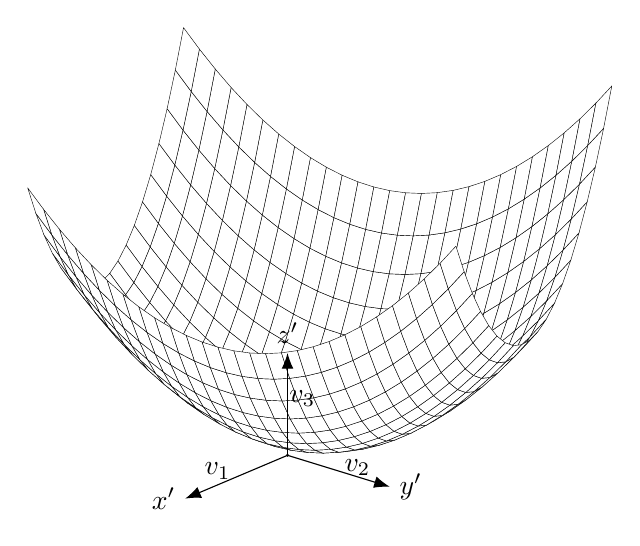
\begin{tikzpicture}
  \begin{axis}[
      hide axis,
      view={20}{25},
      width=9cm, height=9cm,
      domain=-1.6:1.6, y domain=-1.1:1.1,
      samples=28, samples y=20,
      z buffer=sort,
    ]
    \addplot3[surf, shader=faceted, faceted color=black, fill=white,
      opacity=1, line width=0.15pt, mesh/ordering=y varies]
      ({x},{y},{0.6*x^2+1.6*y^2});
  \end{axis}

  \begin{scope}[shift={(3.3cm,1.6cm)}]
    \draw[-{Latex[length=2mm]}] (0,0) -- (-1.3,-0.55) node[left] {$x'$};
    \draw[-{Latex[length=2mm]}] (0,0) -- (1.3,-0.4) node[right] {$y'$};
    \draw[-{Latex[length=2mm]}] (0,0) -- (0,1.3) node[above] {$z'$};
    \node[left=1mm] at (-0.5,-0.2) {$v_1$};
    \node[right=1mm] at (0.5,-0.15) {$v_2$};
    \node[above right=-1mm] at (0,0.6) {$v_3$};
    \fill (0,0) circle (0.6pt);
  \end{scope}
\end{tikzpicture}
\end{document}
